\documentclass[draft]{article}
% The file ijcai17.sty is the style file for IJCAI-17 (same as ijcai07.sty).

%IJCAI 2017 submissions:
%Submitted technical papers must be no longer than seven pages in total: six pages for the main text of the paper (including all figures but excluding references), and one additional page for references. Note that the references page can only include references. DOUBLE BLIND!

\usepackage{ijcai17}

% Use the postscript times font!
\usepackage{times}

\usepackage{latexsym,amssymb,amsmath,amssymb,amsthm,thmtools,mathtools}
\usepackage{xspace}
\usepackage{graphicx}
\usepackage{misc}
\usepackage{mathabx}
\usepackage{color} 
\usepackage{named} 
%\usepackage{pifont}
\usepackage{mathrsfs}
\usepackage{tikz}
\usetikzlibrary{graphs,matrix}
\usepackage[obeyDraft]{todonotes}
\usepackage{standalone}

\usepackage{stackrel}
\usepackage{relsize}

\newcommand{\UMLfull}{UML\ensuremath{_\textit{full}}\xspace}
\newcommand{\UMLbool}{UML\ensuremath{_\textit{bool}}\xspace}
\newcommand{\UMLref}{UML\ensuremath{_\textit{ref}}\xspace}

\newcommand{\UCD}{UCD\xspace}
\newcommand{\UCDs}{UCDs\xspace}
%

%\newcommand{\exptime}{\textsc{ExpTime}\xspace}
\newcommand{\ptime}{\textsc{P}\xspace}
\newcommand{\pspace}{\textsc{PSpace}\xspace}
\newcommand{\nlogspace}{\textsc{NLogSpace}\xspace}
\newcommand{\np}{\textsc{NP}\xspace}

\newcommand{\isa}{\textsc{isa}\xspace}

%\newcommand{\nb}[1]{\textcolor{red}{\textdagger}\marginpar{\scriptsize\raggedright\textcolor{red}{#1}}}
\newcommand{\nb}[1]{\todo[color=red]{#1}\xspace}

\newcommand{\greif}[1]{\ensuremath{\bigocirc#1}}
\newcommand{\lreif}[1]{\ensuremath{\bigodot#1}}

\newcommand\restr[2]{{% we make the whole thing an ordinary symbol
  \left.\kern-\nulldelimiterspace % automatically resize the bar with \right
  #1 % the function
  \vphantom{\big|} % pretend it's a little taller at normal size
  \right|_{#2} % this is the delimiter
  }}
  
\newcommand{\Int}[1]{#1^{\Imc}\xspace}
%\renewcommand\dom{\ensuremath{\Delta^{\Imc}}\xspace}
\renewcommand\dom{\ensuremath{\Delta}\xspace}
\newcommand{\KB}{\ensuremath{\mathcal{KB}}\xspace}
\newcommand{\per}{\mathpunct{\mbox{\bf .}}}
\newcommand{\pth}[2]{\ensuremath{\textsc{path}_{\mathscr{T}}(#1,#2)}\xspace}
\newcommand{\chd}[2]{\ensuremath{\textsc{child}_{\mathscr{T}}(#1,#2)}\xspace}
\newcommand{\A}{\ensuremath{\mathcal{A}}\xspace}
\newcommand{\Ob}{\ensuremath{\mathcal{O}}\xspace}
\newcommand{\Texa}{\ensuremath{\Tmc_{\sf exa}}\xspace}

\DeclareMathOperator*{\RAJoin}{\Join}
\newcommand{\pushright}[1]{\ifmeasuring@#1\else\omit\hfill$\displaystyle#1$\fi\ignorespaces}
\newcommand{\pushleft}[1]{\ifmeasuring@#1\else\omit$\displaystyle#1$\hfill\fi\ignorespaces}
\newcommand{\specialcell}[1]{\ifmeasuring@#1\else\omit$\displaystyle#1$\ignorespaces\fi}

%\renewcommand{\baselinestretch}{0.991}

%%% Color definitions (taken from rgb.tex)
%\definecolor{black}           {rgb}{0.00,0.00,0.00}
%\definecolor{blue}            {rgb}{0.00,0.00,1.00}
%\definecolor{midnightblue}    {rgb}{0.10,0.10,0.44}
%\definecolor{firebrick}       {rgb}{0.70,0.13,0.13}
%\definecolor{forestgreen}     {rgb}{0.13,0.55,0.13}
%\definecolor{gray}            {rgb}{0.75,0.75,0.75}
%\definecolor{gray50}          {rgb}{0.50,0.50,0.50}
%\definecolor{magenta}         {rgb}{1.00,0.00,1.00}
%\definecolor{mediumorchid}    {rgb}{0.73,0.33,0.83}
%\definecolor{mediumslateblue} {rgb}{0.48,0.41,0.93}
%\definecolor{orange}          {rgb}{1.00,0.65,0.00}
%\definecolor{darkorange}      {rgb}{1.00,0.55,0.00}
%\definecolor{orangered}       {rgb}{1.00,0.27,0.00}
%\definecolor{myorange}        {rgb}{1.00,0.40,0.00}
%\definecolor{red}             {rgb}{1.00,0.00,0.00}
%\definecolor{sienna}          {rgb}{0.63,0.32,0.18}
%\definecolor{violetred}       {rgb}{0.82,0.13,0.56}
%\definecolor{white}           {rgb}{1.00,1.00,1.00}
%\definecolor{violetblue}      {rgb}{0.40,0.20,1.00}
%\definecolor{brown}           {rgb}{0.65,0.16,0.16}
%
%\definecolor{myblue}{HTML}{106872}% 007777}%8888}
%\definecolor{mygray}{HTML}{CCCCCC}%6633CC}
%\definecolor{mygrey}{HTML}{cc8879}%6633CC}
%\definecolor{mydarkgray}{HTML}{aaaaaa}
%\definecolor{myorange}{HTML}{cc6877}%995533}%

% #1 - width
% #2 - color
% #3 - text
\newcommand{\coloredboxw}[3]{
  \vspace{0.3cm}
  \begin{tikzpicture}
    \draw let \p1=($(#1,0)-(1,0)$) in node[draw, rectangle, color=#2,
    fill=#2!10!, text=black, rounded corners=10, inner xsep=0.5cm,inner ysep=1mm] {
      \begin{minipage}[t]{\x1}
        #3
      \end{minipage}};
  \end{tikzpicture}
  \vspace{-0.5cm}
}

% #1 - color
% #2 - text
%\newcommand{\coloredbox}[2]{
%  \coloredboxw{\linewidth}{#1}{#2}
%}
%
%%%%%%%%% Colors
%\newcommand {\bblu}[1]  {\color{blue}{\sf #1}}
%\newcommand {\bred}[1]  {\color{red}\sf{#1}}
%\newcommand {\bgreen}[1]  {\color{green}\sf{#1}}
%
%\newcommand{\bb}[1]{\textcolor{blue}{#1}}
%\newcommand{\bbd}[1]{\textcolor{midnightblue}{#1}}
%\newcommand{\rr}[1]{\textcolor{red}{#1}}
%\newcommand{\mm}[1]{\textcolor{magenta}{#1}}
%\newcommand{\nn}[1]{\textcolor{black}{#1}}
%\renewcommand{\gg}[1]{\textcolor{forestgreen}{#1}}
%\newcommand{\gr}[1]{\textcolor{gray50}{#1}}
%\renewcommand{\ss}[1]{\textcolor{sienna}{#1}}
%\newcommand{\oo}[1]{\textcolor{myorange}{#1}}
%\newcommand{\vv}[1]{\textcolor{violetred}{#1}}
\newcommand{\ww}[1]{\textcolor{white}{#1}}
%\newcommand{\bl}[1]{\textcolor{mediumslateblue}{#1}}
%\newcommand{\vb}[1]{\textcolor{violetblue}{#1}}
%\newcommand{\fb}[1]{\textcolor{firebrick}{#1}}

\thickmuskip=3mu plus 2mu minus 2mu

%%%% Theorems
\declaretheorem{theorem}
\declaretheorem{lemma}
\declaretheorem{corollary}

\newtheorem{proposition}{Proposition}
\newtheorem{property}{Property}
\newtheorem{definition}{Definition}
\newtheorem{example}{Example}

%%%%%%%%%%%%%%%%%%%%%%%%%%%%%%%%%%%%%%%%%%%%%%%%%%%%%%%%%%%%%%%%%%%%%%
\title{A Decidable Very Expressive \textit{n}-ary Description Logic for Database Applications}

%%% blind review!
%\author{Alessandro Artale, Enrico Franconi, Rafael Pe\~naloza, Francesco Sportelli\\
%KRDB Research Centre, 
%Free University of Bozen-Bolzano, Italy\\
%\texttt{\{artale,franconi,penaloza,sportelli\}@inf.unibz.it}
%}

\begin{document}

\date{}
\maketitle

%%%%%%%%%%%%%%%%%%%%%%%%%%%%%%%%%%%%%%%%%%%%%%%%%%%%%%%%%%%%%%%%%%%%%%

\begin{abstract}
We introduce \DLRp{}\negmedspace, an extension of the $n$-ary propositionally closed description logic \DLR to deal with attribute-labelled tuples (generalising the positional notation), projections of relations (expressing inclusion dependencies), functional, key, and external uniqueness dependencies, identification constraints, and global and local objectification of relations. A \DLRp knowledge base includes TBox and ABox axioms. A simple syntactic restriction on the appearance of projections sharing common attributes in the knowledge base makes reasoning in the language decidable with the same computational complexity as \DLR. 
The obtained \DLRpm $n$-ary description logic is able to encode more thoroughly conceptual data models such as EER, UML, ORM.
\end{abstract}

%%%%%%%%%%%%%%%%%%%%%%%%%%%%%%%%%%%%%%%%%%%%%%%%%%%%%%%%%%%%%%%%%%%%%%
%%%%%%%%%%%%%%%%%%%%%%%%%%%%%%%%%%%%%%%%%%%%%%%%%%%%%%%%%%%%%%%%%%%%%%

\begin{figure*}
	[t] 
%	\begin{center}
	\centering
		\renewcommand{\arraystretch}{1.1} 
		$
		\begin{array}{r@{\hspace{2ex}}c@{\hspace{2ex}}l} 
			C & \to & \top\ \mid\ \bot\ \mid\ C\!N\ \mid\ \neg C\ \mid\ C_{1}\sqcap C_{2}\ \mid\ C_{1}\sqcup C_{2}\ \mid\ \EXISTR{q}{U_i} R\ \mid\ \greif{R}\ \mid\ \lreif{R\!N}\\
			%
			R & \to & R\!N\ \mid\ R_1\setminus R_2\ \mid\ R_{1}\sqcap R_{2}\mid\ R_{1}\sqcup R_{2}\mid\ \selects{U_i}{C}{R}\ \mid\ \EXISTR{q}{U_1,\ldots,U_k} R\\
			\varphi & \to & C_1\sqsubseteq C_2\ \mid\ R_1\sqsubseteq R_2 \mid C\!N(o) \mid R\!N(U_1\!:\!o_1,\ldots,U_n\!:\!o_n) \mid o_1 = o_2 \mid o_1 \neq o_2 \\
			\vartheta & \to & U_1 \rightleftarrows U_2
		\end{array}
		$ 
		\vspace*{-2ex}
		\renewcommand{\arraystretch}{1} 
%	\end{center}
	\caption{\label{fig:dlrp} Syntax of \DLRp.} 
\end{figure*}

%%%%%%%%%%%%%%%%%%%%%%%%%%%%%%%%%%%%%%%%%%%%%%%%%%%%%%%%%%%%%%%%%%%%%%
%%%%%%%%%%%%%%%%%%%%%%%%%%%%%%%%%%%%%%%%%%%%%%%%%%%%%%%%%%%%%%%%%%%%%%
\section{Introduction}

We introduce the new description logic \DLRp{}\negmedspace extending the $n$-ary description logics \DLRID~\cite{CalvaneseGL01}, itself based on the description logic \DLR~\cite{HorrocksSTT00,Calvanese:et:al:TOCL-2008}, in order to capture more database oriented constraints.
%
\nb{Should we not cite the DL paper?} % \cite{DBLP:conf/dlog/ArtaleF16}
%
While \DLRID is a rather expressive logic, it lacks a number of expressive means that can be added without increasing the complexity of reasoning---when used in a carefully controlled way.

The added expressivity is motivated by the increasingly use of description logics as an abstract conceptual layer over relational databases, both to reason over such conceptual models during the database design phase (see, e.g., works as~\cite{calvanese:et:al:98a,BeCD05-AIJ-2005,ACKRZ:er07,artale:franconi:john09,TomanW09,ACI:er10,DBLP:conf/otm/FranconiMS12}) and to answer ontology-mediated queries over databases (see, e.g, works as~\cite{ACKZ:jair09,DBLP:journals/jair/FranconiKN13}).
%as witnessed by the W3C standard OWL 2 QL effort~\cite{OWL2QL}.

To describe the added expressivity of \DLRp we consider the scenario where the following verbs are modelled: a generic ${\tt TransitiveVerb}$ and two specific verbs as ${\tt Love}$ and ${\tt Kill}$. Then, in \DLRp the following constraints that are common both in databases and in data model can be captured:

\begin{itemize}
	
	\item Instances of relations are so called \emph{attribute-labelled tuples}, i.e., tuples such that their components are identified by an attribute and not by a position in the tuple. Thus, the three verbs can be captured in \DLRp with the following relations:
%
  \begin{align*}
    &{\tt TransitiveVerb (Agent, Patient, When)},\\
    &{\tt Love(Lover, Loved, When, How)},\\
    &{\tt Kill(Killer,Killed,When,Location,Tool)}.
  \end{align*}
%
A possible instance of the ${\tt Kill}$ event has the form:
%
\begin{multline*}
  \langle {\tt Killer}\!:\!\textit{John},  {\tt Killed}\!:\!
  \textit{Mary}, {\tt When}:\textit{23.11.1974}\\
    {\tt Location}\!:\!\textit{NY}, {\tt Tool}\!:\!\textit{gun}\rangle.
\end{multline*}
%
% the semantics is based on attribute-labelled tuples: an element
%   of a tuple is identified by an attribute and not by its position in
%   the tuple, e.g., the relation \texttt{Person} has attributes
%   \texttt{firstname}, \texttt{lastname},
%   \texttt{age}, \texttt{height} with instance:\\
%   \texttt{$\langle$ firstname: Enrico, lastname: Franconi, age: 53,
%     height: 1.90$\rangle$};
%
	\item \emph{Renaming of attributes} is possible, e.g., to recover the positional semantics. In our example, we can rename the ${\tt TransitiveVerb}$ attributes into the positional attributes with the following:
%
  \begin{align*}
  {\tt Agent, Patient, When}\rightleftarrows \texttt{1,2,3}.
  \end{align*}
%
	\item \emph{Relation projections} (with the same meaning of projections in databases) allow to form new relations by projecting a given relation on some of its attributes. For example, to capture that every triple of the form ${\tt Lover, Loved, When}$ is also a ${\tt TransitiveVerb}$ we can project the ${\tt Love}$ relation and add the axiom (inclusion dependency):
%
  \begin{align*}
    \ATLEASTRS{{\tt Lover, Loved,When}}{\tt Love} \sqsubseteq {\tt TransitiveVerb}.
  \end{align*}
%
% it can express projections of relations, and therefore inclusion dependencies, e.g.,
% $\ATLEASTRS{\texttt{firstname,lastname}}\texttt{Student}\sqsubseteq\ATLEASTRS{\texttt{firstname,lastname}}\texttt{Person}$;
%
	\item \emph{Functional dependencies} and, in particular, \emph{multiple-attribute keys} can be expressed via the multiple-attribute cardinalities construct. Therefore, e.g., to express that the pair ${\tt Killer, Killed}$ is a key for the ${\tt Kill}$ relation can be captured by the following axiom:
%
  \begin{multline*}
    \ATLEASTRS{{\tt Killer, Killed}}{\tt Kill} \sqsubseteq \\
    \exists^{\leq 1}[{\tt Killer, Killed}]{\tt Kill}.
  \end{multline*}
%
% the functional dependency from \texttt{firstname,} \texttt{lastname} to \texttt{age} in \texttt{Person} can be written as:\\
% $\exists[\texttt{firstname,lastname}] \texttt{Person} \sqsubseteq$ 
% \hspace{2em} $\exists^{\leq 1}[\texttt{firstname,lastname}](\exists[\texttt{firstname,lastname,age}] \texttt{Person})$;
%
	\item \emph{Local and global objectification} (the last one is also known as reification) allow to create a new concept starting from a relation where relation tuples are identified either by a unique global identifier or by an identifier which is unique only within the interpretation of a relation, depending whether global or local objectification, respectively, is used. While global objectification corresponds to the well known reification construction, we show an example of the local objectification. Consider the relations ${\tt OwnsCar(Name, Car)}$ and ${\tt DrivesCar(Name, Car)}$ and assume that to drive a car you should also own it, i.e., ${\tt DrivesCar\sqsubseteq OwnsCar}$. By using classical reification to capture the events of driving and owing a car we logically imply a subsumption between the two reified events. On the other hand, if we use local objectification to generate the two events the subsumption is no more implied and actually the two events can also be disjoint (as they should be considered).

% it can express global and local objectification (also known as reification): a tuple may be identified  by a unique global identifier, or by an identifier which is unique only within the interpretation of a relation, e.g., to identify the name of a person we can write 
% $\texttt{Name}\sqsubseteq\lreif{\exists[\texttt{firstname,lastname}] \texttt{Person}} $.

\end{itemize}

Besides a TBox, \DLRp also expresses factual knowledge via an ABox where objects and labelled-tuples are asserted to belong to concepts and relations, respectively. 

While \DLRp is undecidable due to the possibility to express arbitrary functional and inclusion dependencies~\cite{Mitchell83,ChandraV85} we show how a simple syntactic condition on the appearance of projections in the knowledge base makes the language decidable. The result of this restriction is a new language called \DLRpm{}\negmedspace. We prove that \DLRpm{}\negmedspace, while preserving most of the \DLRp expressivity, has a reasoning problem whose complexity does not increase w.r.t. the computational complexity of the basic \DLR language. Furthermore, \DLRpm is able to correctly express the UML/EER conceptual data models as introduced in~\cite{BeCD05-AIJ-2005,ACKRZ:er07} and the ORM conceptual data model as introduced in~\cite{DBLP:conf/otm/FranconiM13}.

%%%%%%%%%%%%%%%%%%%%%%%%%%%%%%%%%%%%%%%%%%%%%%%%%%%%%%%%%%%%%%%%%%%%%%
%%%%%%%%%%%%%%%%%%%%%%%%%%%%%%%%%%%%%%%%%%%%%%%%%%%%%%%%%%%%%%%%%%%%%%


\section{The Description Logic \DLRp}
\label{sec:syntax}

We first define the syntax of \DLRp. A \DLRp \emph{signature} is a tuple $\mathcal{L}=(\mathcal{C},\mathcal{R},\mathcal{O},\mathcal{U},\tau)$ where $\mathcal{C}$, $\mathcal{R}$, $\mathcal{O}$ and $\mathcal{U}$ are finite, mutually disjoint sets of \emph{concept names}, \emph{relation names}, \emph{individual names}, and \emph{attributes}, respectively, and $\tau$ is a \emph{relation signature} function, associating a set of attributes to each relation name $\tau(R\!N)=\{U_1,\ldots,U_n\}\subseteq \Umc$ with $n\geq 2$.

The syntax of concepts $C$, relations $R$, formulas $\varphi$, and attribute renaming axioms $\vartheta$ is given in Figure~\ref{fig:dlrp}, where $C\!N\in\mathcal{C}$, $R\!N\in\mathcal{R}$, $U\in\mathcal{U}$, $o\in \Ob$, $q$ is a positive integer and $2\leq k < \textsc{arity}(R)$.  
The \emph{arity} of a relation  $R$ is the number of the attributes in its signature; i.e., $\textsc{arity}(R)=\left|\tau(R)\right|$, where we extend the signature function $\tau$ to arbitrary relations as specified in Figure~\ref{fig:syn:tau}.
Notice that, while global objectification ($\greif{R}$) can be applied to arbitrary relations, local ones ($\lreif{R\!N}$) can be applied just to relation names. We use the shortcut $\exists[U_1,\ldots,U_k] R$ for $\exists^{\geq 1}[U_1,\ldots,U_k] R$ for $k\geq 1$.

%
\begin{figure}[t] 
	\centering
	\resizebox{\columnwidth}{!}{
%		\renewcommand{\arraystretch}{1.2} 
		$ { 
		\begin{array}{r@{\hspace{1ex}}l@{\hspace{3ex}}l@{\hspace{.3ex}}} 
			\tau(R_1\setminus R_2) = & \tau(R_1) & \text{if } \tau(R_1)=\tau(R_2)\\
			\tau(R_{1}\sqcap R_{2}) = & \tau(R_1) & \text{if } \tau(R_1)=\tau(R_2)\\
			\tau(R_{1}\sqcup R_{2}) = & \tau(R_1) & \text{if } \tau(R_1)=\tau(R_2)\\
			\tau(\selects{U_i}{C}{R}) = & \tau(R) & \text{if } U_i\in\tau(R)\\
			\tau(\EXISTR{q}{U_1,\ldots,U_k} R) = & \{U_1,\ldots,U_k\} & \text{if } \{U_1,\ldots,U_k\}\subset \tau(R)\\
			\tau(R) = & \emptyset & \text{otherwise} 
		\end{array}
		}$ 
%		\renewcommand{\arraystretch}{1} 
	}
%	\end{center}
	\vspace*{-2ex}
	\caption{\label{fig:syn:tau} The signature of \DLRp relations.} 
\end{figure}
%

A \DLRp \emph{TBox} \Tmc is a finite set of \emph{concept inclusion} axioms of the form $C_1\sqsubseteq C_2$ and \emph{relation inclusion} axioms of the form $R_1\sqsubseteq R_2$. We use $X_1\equiv X_2$ as a shortcut for the two axioms $X_1\sqsubseteq X_2$ and $X_2\sqsubseteq X_1$. A \DLRp \emph{ABox} \Amc is a finite set of \emph{concept instance} axioms of the form $C\!N(o)$, \emph{relation instance} axioms of the form $R\!N(U_1\!:\!o_1,\ldots,U_n\!:\!o_n)$, and \emph{same/distinct individual} axioms of the form $o_1 = o_2$ and $o_1 \neq o_2$, with $o_i\in\Ob$. Restricting ABox axioms to concept and relation names only does not affect the expressivity of \DLRp due to the availability of TBox axioms.

A set of renaming axioms forms a \emph{renaming schema}, which induces an equivalence relation $(\rightleftarrows,\mathcal{U})$ over the attributes $\mathcal{U}$, providing a partition of $\mathcal{U}$ into equivalence classes each one representing the alternative ways to name attributes. We write $[U]_\Re$ to denote the equivalence class of the attribute $U$ w.r.t. the equivalence relation $(\rightleftarrows,\mathcal{U})$. We allow only \emph{well founded} renaming schemas; that is, schemas such that each equivalence class $[U]_\Re$ in the induced equivalence relation never contains two attributes from the same relation signature. 
%
We use the shortcut $U_1\ldots U_n\rightleftarrows U'_1\ldots U'_n$ to group many renaming axioms with the obvious meaning that $U_i\rightleftarrows U'_i$, for all $i=1,\ldots, n$.

%The selection expression $\selects{U_i}{C}{R\!N}$ denotes the
%relation $R\!N$ where the attribute $U_i$ is restricted to the
%concept $C$.
%%
%Global and local \emph{objectification} (also known as reification) of
%relations are denoted as $\greif{R}, \lreif{R\!N}$,
%respectively.
%%
%The \emph{unary projection} expression, $\EXISTR{q}{U_i} R$, denotes a
%concept expression as a generalisation with cardinalities of the unary
%projection operator over the attribute $U_i$ of the relation $R$; we
%denote with $\exists[U_i]R$ the plain unary projection. In \DLRp we
%can express $n$-ary projections (possibly with cardinalities) denoted
%as $\EXISTR{q}{U_1,\ldots,U_k} R$.
%%
%% With $\rho_{U_1/U'_1,\ldots,U_l/U'_l}R$ we denote the relation $R$
%% where attributes $\{U_1,\ldots,U_l\}$ are renamed as
%% $\{U'_1,\ldots,U'_l\}$. 
%
The renaming schema reconciles the named attribute and the positional perspectives on relations (see, e.g.,~\cite{Kanellakis:1990:chapter}). They are crucial when expressing both inclusion axioms and set operators ($\sqcap,~\sqcup,~\setminus$) between relations, which make sense only over \emph{union compatible} relations. Two relations $R_1,R_2$ are union compatible if their signatures are equal up to the attribute renaming induced by the renaming schema $\Re$, namely, $\tau(R_1)=\{U_1,\ldots,U_n\}$ and $\tau(R_2)=\{V_1,\ldots,V_n\}$ have the same arity $n$ and $[U_i]_\Re=[V_i]_\Re$ for each $1\leq i\leq n$. Notice that through the renaming schema, relations can use just local attribute names that can then be renamed when composing relations. Also note that it is obviously possible for the same attribute to appear in the signature of different relations.

%
A \DLRp knowledge base (KB) $\mathcal{KB}=(\Tmc\!,\Amc,\Re)$ is composed by a TBox \Tmc, an ABox \Amc, and a renaming schema $\Re$.

%\vspace{2ex}
%
%To show the expressive power of the language, let us consider the following example with tree relation names $R_1, R_2$ and $R_3$ with the following signature:
%%
%\begin{align*}
%  \tau(R_1)  &= \{U_1,U_2,U_3,U_4,U_5\}\\
%  \tau(R_2)  &= \{V_1,V_2,V_3,V_4,V_5\}\\
%  \tau(R_3)  &= \{W_1,W_2,W_3,W_4\}
%\end{align*}
%%
%To state that $\{U_1,U_2\}$ is the \emph{multi-attribute key} of $R_1$ we add the axiom:
%  \begin{align*}
%    \exists[U_1,U_2] R_1 \sqsubseteq \exists^{\leq 1}[U_1,U_2] R_1
%  \end{align*}
%%
%where $\exists[U_1,\ldots,U_k] R$ stands for $\exists^{\geq 1}[U_1,\ldots,U_k] R$. To express that there is a \emph{functional dependency} from the attributes $\{V_3,V_4\}$ to the attribute $\{V_5\}$ of $R_2$ we add the axiom:
%\begin{align}\label{funct-dep}
%      \exists[V_3,V_4] R_2 \sqsubseteq \exists^{\leq 1}[V_3,V_4](\exists[V_3,V_4,V_5] R_2)
%\end{align}
%%
%The following axioms express that $R_2$ is a sub-relation of $R_1$ and
%that a projection of $R_3$ is a sub-relation of a projection of $R_1$,
%together with the corresponding axioms for the
%renaming schema to explicitly specify the % exact behaviour
%correspondences between the attributes of the two inclusion dependencies:
%%2
%\begin{align*}
%  R_2 &\sqsubseteq R_1\\
%  \exists[W_1,W_2,W_3] R_3 &\sqsubseteq \exists[U_3,U_4,U_5] R_1\\
%  V_1V_2V_3V_4V_5 &\rightleftarrows U_1U_2U_3U_4U_5 \\
%  W_1W_2W_3 &\rightleftarrows U_3U_4U_5
%\end{align*}

\begin{example}
\label{exa:basic}
Consider the relation names $R_1, R_2$ where
%
%\begin{align*}
 $\tau(R_1)  = \{W_1,W_2,W_3,W_4\}$,
%  $\tau(R_1)  = \{U_1,U_2,U_3,U_4,U_5\}$,
 $\tau(R_2)  = \{V_1,V_2,V_3,V_4,V_5\}$,
%\end{align*}
%
and the renaming axiom 
$W_1W_2W_3 \rightleftarrows V_3V_4V_5$.
The TBox \Texa consists of the axioms:
%
 \begin{align}
   R_2 \sqsubseteq {} & R_1 \label{isaR}\\
   \exists[W_1,W_2] R_1 \sqsubseteq {} & \exists^{\leq 1}[W_1,W_2] R_1 \label{key} \\
     \exists[V_3,V_4] R_2 \sqsubseteq {} & \exists^{\leq 1}[V_3,V_4](\exists[V_3,V_4,V_5] R_2) \label{funct-dep} \\
 \exists[W_1,W_2,W_3] R_1 \sqsubseteq {} & \exists[V_3,V_4,V_5] R_2 \label{subrelation}.
 \end{align}
%
 Intuitively, the axiom~\eqref{key}
 expresses that $W_1,W_2$ form a multi-attribute key for $R_1$;
 \eqref{funct-dep} introduces a functional dependency in the relation
 $R_2$ where the attribute $V_5$ is functionally dependent from
 attributes $V_3, V_4$, and \eqref{subrelation} states an inclusion
 between two projections of the relation names $R_1, R_2$ based on
 the renaming schema axiom.
\end{example}

%%%%%%%%%%%%%%%%%%%%%%%%%%%%%%%%%%%%%%%%%%%%%%%%%%%%%%%%%%%%%%%%%%%%%%
%%%%%%%%%%%%%%%%%%%%%%%%%%%%%%%%%%%%%%%%%%%%%%%%%%%%%%%%%%%%%%%%%%%%%%

%\section{Semantics}  

The semantics of \DLRp uses of the notion of \emph{labelled tuples} over a domain $\Delta$: a 
\emph{$\mathcal{U}$-labelled tuple over $\Delta$} (or \emph{tuple} for short) is a function 
$t \colon \mathcal{U} \to \Delta$. For $U\in \mathcal{U}$, we write $t[U]$ to refer to the domain element ${d\in \Delta}$ 
labelled by $U$, if the function $t$ is defined for $U$---that is, if the attribute $U$ is a label of the tuple $t$. 
Given $d_1,\dots,d_n\in \Delta$, the expression ${\langle U_1\colon d_1,\ldots,U_n\colon d_n\rangle}$ stands for the 
tuple $t$ such that ${t[U_i]=d_i}$, for ${1\leq 1\leq n}$. 
% and the expression ${{U_i:d_i}\in t}$ stands for ${t[U_i]=d_i}$, for ${1\leq 1\leq n}$.
The \emph{projection} of the tuple $t$ over the attributes ${U_1,\ldots,U_k}$ (i.e., the function $t$ 
restricted to be undefined for the labels not in ${U_1,\ldots,U_k}$)
is denoted by ${t[U_1,\ldots,U_k]}$. 
The relation signature function $\tau$ can be applied also to labelled
tuples to obtain the set of labels on which the tuple is defined.
$T_\Delta(\mathcal{U})$ denotes the set of all $\mathcal{U}$\mbox{-}labelled tuples over $\Delta$.

A \DLRp \emph{interpretation} is a tuple $\Imc = (\dom, \cdot^\Imc, \rho, \imath, L)$ consisting of a nonempty 
\emph{domain} $\dom$, an \emph{interpretation function} $\cdot^\Imc$, a \emph{renaming function} $\rho$, a \emph{global objectification function} $\imath$, and a family $L$ containing one \emph{local objectification function} 
$\ell_{R\!N_i}$ for each named relation $R\!N_i\in\mathcal{R}$.

The renaming function $\rho$ is a total function ${\rho:\mathcal{U}\to\mathcal{U}}$ representing a canonical renaming 
for all attributes. We use $\rho(\{U_1,\ldots,U_k\})$  to denote $\{\rho(U_1),\ldots,\rho(U_k)\}$.
%
The global objectification function is an injective function, ${\imath:T_{\dom}(\Umc) \to \dom}$, associating a \emph{unique} global identifier to each tuple.
%
% and\nb{A: dobbiamo re-introdurre} it is such that $\imath(\langle U:d \rangle)=d$, for any
% $U\in\Umc$ and $d\in\dom$, namely it identifies unary tuples with
% their value.
The local objectification functions, ${\ell_{R\!N_i}:T_{\dom}(\Umc) \to \dom}$, are associated to each relation name in the signature, and as the global objectification function they are injective: they associate an identifier---which is guaranteed to be unique only within the interpretation of a relation name---to each tuple.
%and they are such that $\ell_{R\!N_i}(\langle U:d \rangle)=d$ for any $U\in\Umc$ and $d\in\dom$.
The interpretation function $\cdot^\Imc$ assigns a domain element to each individual $o^{\mathcal{I}}\in\dom$, a set of domain elements to each concept name $C\!N^{\mathcal{I}}\subseteq \dom$, and a set of $\Umc$-labelled tuples over $\dom$ to each relation name conforming with its signature and to the renaming function $R\!N^{\mathcal{I}}\subseteq T_{\dom}(\{\rho(U)\mid U\in\tau(R\!N)\})$. Note that the unique name assumption is not enforced.
%
The interpretation function $\cdot^\Imc$ is unambiguously extended over concept and relation expressions as specified in Figure~\ref{fig:sem:dlrp}.%
%
\begin{figure}[t] 
	\centering
		\resizebox{\columnwidth}{!}{
		$ 
		\begin{array}{@{}r@{\hspace{1ex}}l@{}} 
			\Int{\top} = & \dom\\
			%
			\Int{\bot} = & \emptyset\\
			%
			\Int{(\neg C)} = & \Int{\top} \setminus \Int{C}\\
			%
			\Int{(C_{1}\sqcap C_{2})} = & \Int C_{1} \cap \Int C_{2}\\
			%
			\Int{(C_{1}\sqcup C_{2})} = & \Int C_{1} \cup \Int C_{2}\\
			%
			\Int{(\EXISTR{q}{U_i} R)} = & \{d\in\dom\mid~\left|\{t\in\Int R\mid t[\rho(U_i)]=d\}\right| \lesseqgtr q \}\\
			%
			\Int{(\greif{R})} = & \{d\in \dom \mid d=\imath(t) \land t\in \Int{R}\}\\
			%
			\Int{(\lreif{R\!N})} = & \{d\in \dom \mid d=\ell_{R\!N}(t)\land t\in \Int{R\!N}\}\\
			%
			\Int{(R_1\setminus R_2)} = & \Int R_{1} \setminus \Int R_{2}\\
			%
			\Int{(R_{1}\sqcap R_{2})} = & \Int R_{1} \cap \Int R_{2}\\
			%
			\Int{(R_{1}\sqcup R_{2})} = & \{t\in\Int R_{1}\cup\Int R_{2}\mid \rho(\tau(R_1))= \rho(\tau(R_2))\}\\
			%
			\Int{(\selects {U_i}{C}{R})} = & \{
			t\in\Int{R} \mid t[\rho(U_i)]\in\Int{C}\} \\
			%
			\Int{(\EXISTR{q}{U_1,\ldots,U_k} R)} = & \{
			\langle \rho(U_1):d_1,\ldots,\rho(U_k):d_k\rangle \in T_{\dom}(\{\rho(U_1),\ldots,\rho(U_k)\}) \mid \\
			& \left|\{t\in\Int R \mid t[\rho(U_1)]=d_1,\ldots,t[\rho(U_k)]=d_k\}\right| \lesseqgtr q \}
		\end{array}
		$
		}
%	\end{center}
	\vspace*{-1.5ex}
	\caption{Semantics of \DLRp expressions.} 
	\label{fig:sem:dlrp}
\end{figure}

The interpretation $\Imc$ satisfies the concept inclusion axiom $C_1\sqsubseteq C_2$ if $\Int C_1\subseteq \Int C_2$, and the relation inclusion axiom $R_1\sqsubseteq R_2$ if $\Int R_1\subseteq \Int R_2$. It satisfies the concept instance axiom $C\!N(o)$ if $\Int o\in \Int {C\!N}$\!, the relation instance axiom $R\!N(U_1\!:\!o_1,\ldots,U_n\!:\!o_n)$ if ${\langle \rho(U_1)\colon\Int{o_1},\ldots,\rho(U_n)\colon\Int{o_n}\rangle}\in \Int {R\!N}$, and the axioms $o_1 = o_2$ and $o_1 \neq o_2$ if $\Int{o_1} = \Int{o_2}$, and $\Int{o_1} \neq \Int{o_2}$, respectively. $\Imc$ satisfies a renaming schema $\Re$ if
%the renaming function $\rho$ renames the attributes in a consistent way with respect to $\Re$, namely if
%$$\forall U\per\rho(U)\in[U]_\Re\land\forall V\in [U]_\Re\per\rho(U)=\rho(V).$$
for every $U,V\in\mathcal{U}$, (i) $\rho(U)\in[U]_\Re$, and (ii) if $V\in [U]_\Re$, then $\rho(U)=\rho(V)$. 
%
\Imc is a \emph{model} of the KB $(\mathcal{T}\!,\mathcal{A},\Re)$ if it satisfies all the axioms in the TBox $\mathcal{T}$ and in the ABox $\mathcal{A}$, and the renaming schema $\Re$.

\emph{KB satisfiability} refers to the problem of deciding the existence of a model of a given KB;
\emph{concept satisfiability} (resp. \emph{relation satisfiability}) is the problem of deciding whether there is a model of 
the KB that assigns a non-empty extension to a given concept (resp. relation); and 
\emph{entailment} is to check whether the KB logically implies an axiom, that is, whether all models of the KB are also models of the axiom.
%
For instance, from the TBox in Example~\ref{exa:basic} we can entail that
$V_3,V_4$ are a key for the relation $R_2$:
%
$$
 \Texa\models \exists[V_3,V_4] R_2 \sqsubseteq \exists^{\leq 1}[V_3,V_4] R_2.
$$
%
%
All the decision problems can be reduced to KB satisfiability.
\begin{lemma}
In \DLRp, concept and relation satisfiability and entailment are reducible to KB satisfiability.
%	The problems of concept and relation satisfiability and of entailment in \DLRp are reducible to \DLRp KB satisfiability.
\end{lemma}

%%%%%%%%%%%%%%%%%%%%%%%%%%%%%%%%%%%%%%%%%%%%%%%%%%%%%%%%%%%%%%%%%%%%%%%%%%

\section{Expressiveness of \DLRp}
\label{sec:expressivity}

\DLRp is a very expressive description logic capable of asserting several kinds of constraints that are important in the context of relational databases, such as \emph{inclusion dependencies} (inclusion axioms among arbitrary
projections of relations), \emph{equijoins}, \emph{functional dependency} axioms, \emph{key} axioms, \emph{external uniqueness} axioms,  \emph{identification} axioms, and \emph{path functional dependencies}.

An \emph{equijoin} among two relations with disjoint signatures is the set of all combinations of tuples in the relations that are equal on their selected attribute names. Let $R_1,R_2$ be relations with 
$\tau(R_1)=\{U,U_1,\ldots,U_{n_1}\}$ and $\tau(R_2)=\{V,V_1,\ldots,V_{n_2}\}$; their equijoin over $U$ 
and $V$ is the relation  $R = R_1\!\stackrel[U=V]{}{\mathlarger{\mathlarger{\mathlarger{\bowtie}}}}\!R_2$ with 
signature $\tau(R)=\tau(R_1)\cup\tau(R_2)\setminus\{V\}$, %\{U,U_1,\ldots,U_{n_1},V_1,\ldots,V_{n_2}\}$, 
which is expressed by the \DLRp axioms:
%
\renewcommand*{\arraystretch}{1.3}
$$\begin{array}{l}
\exists[U,U_1,\ldots,U_{n_1}]R  \equiv {} \selects{U}{(\exists[U]R_1\sqcap \exists[V]R_2)}{R_1} \\
\exists[V,V_1,\ldots,V_{n_2}]R \equiv {} \selects{V}{(\exists[U]R_1\sqcap \exists[V]R_2)}{R_2}
\\  U\rightleftarrows V~.
\end{array}
\renewcommand*{\arraystretch}{1}
$$

A \emph{functional dependency} axiom $(R:U_1\ldots U_j \rightarrow U)$ states that the values of the attributes $U_1\ldots U_j$ uniquely determine the value of the attribute $U$ in the relation $R$. 
Formally, the interpretation $\Imc$ satisfies this functional dependency axiom %$(R:U_1\ldots U_j \rightarrow U)$ 
if, for all tuples $s,t\in R^\Imc$, $s[U_1] = t[U_1], \ldots, s[U_j] = t[U_j]$ imply $s[U] = t[U]$. Functional dependency axioms are also called \emph{internal uniqueness} axioms~\cite{halpin2008}. Functional dependencies can be expressed in 
\DLRp{}\negmedspace, assuming that $\{U_1,\ldots, U_j, U\}\subseteq \tau(R)$, with the axiom:
%
$$\exists[U_1,\ldots, U_j]R\sqsubseteq\exists^{\leq 1}[U_1,\ldots, U_j](\exists[U_1,\ldots, U_j, U] R).$$
%
A special case of functional dependencies are \emph{key} axioms $(R:U_1\ldots U_j \rightarrow R)$, which state 
that the values of the key attributes $U_1\ldots U_j$ of a relation $R$ uniquely identify tuples in $R$. A key axiom can be expressed in \DLRp, assuming that $\{U_1\ldots U_j\}\subseteq\tau(R)$, with the axiom:
%
$$\exists[U_1,\ldots, U_j]R\sqsubseteq\exists^{\leq 1}[U_1,\ldots, U_j]R.$$

The \emph{external uniqueness} axiom $([U^1]R_1\downarrow\ldots \downarrow [U^h]R_h)$ states that the join $R$ of the relations $R_1,\ldots,R_h$ via the attributes $U^1,\ldots,U^h$ has the joined attribute functionally dependent on all the others~\cite{halpin2008}. This can be expressed in \DLRp with the axioms:
%
%\vspace*{-2mm}
\renewcommand*{\arraystretch}{1.3}
$$\begin{array}{l}
R\equiv {} R_1\!\stackrel[U^1=U^2]{}{\mathlarger{\mathlarger{\mathlarger{\bowtie}}}}\cdots\stackrel[U^{h-1}=U^{h}]{}{\mathlarger{\mathlarger{\mathlarger{\bowtie}}}}\!R_h\\
R: {}  U^1_{1},\ldots, U^1_{n_1},\ldots,U^h_{1},\ldots, U^h_{n_h} \rightarrow U^1
\end{array}
\renewcommand*{\arraystretch}{1}
%\vspace*{-2mm}
$$
%
where $\tau(R_i)=\{U^i,U^i_1,\ldots, U^i_{n_i}\}, 1\le i\le h$, and $R$  with 
%the signature
%
$\tau(R)=\{U^1,U^1_{1},\ldots, U^1_{n_1},\ldots,U^h_{1},\ldots, U^h_{n_h}\}$ is a new relation name.

\emph{Identification} axioms as defined in \DLRID~\cite{CalvaneseGL01}
(an extension of \DLR with functional dependencies and identification
axioms) are a variant of external uniqueness axioms, constraining only
the elements of a concept $C$; they can be expressed in \DLRp with the
axiom:
%
$$
[U^1]\selects{U_1}{C}{R_1}\downarrow\ldots \downarrow [U^h]\selects{U_h}{C}{R_h}.
$$

% The DL \DLRID introduced by~\citeauthor{CalvaneseGL01} extends \DLR with functional dependencies 
% and identification axioms, and is therefore included in \DLRp{}\negmedspace. 
% It is also easy to see that \DLRp includes \ALCQI.

%Summing up, \DLRp extends the description logic \DLRID, which obvioulsy includes \ALCQI. Furthermore, 
\emph{Path functional dependencies}---as defined in the $\mathcal{CFD}$ family of description logics ~\cite{TomanW09}---can be expressed in \DLRp as identification axioms involving joined sequences of functional binary relations.

The rich set of constructors in \DLRp allows us to extend the known mappings in description logics of popular conceptual data models. The EER mapping as introduced in~\cite{ACKRZ:er07} can be extended to deal with multi-attribute keys (by using identification axioms) and named roles in relations; the ORM mapping as introduced in~\cite{DBLP:conf/otm/FranconiMS12,DBLP:conf/otm/FranconiM13,DBLP:conf/otm/SportelliF16} can be extended to deal with arbitrary subset and exclusive relation constructs (by using inclusions among global objectifications of projections of relations), arbitrary internal and external uniqueness constraints, arbitrary frequency constraints (by using projections), local objectification, named roles in relations, and fact type readings (by using renaming axioms); the UML mapping as introduced in~\cite{BeCD05-AIJ-2005} can be fixed\nb{how to say this without offending?} to deal properly with association classes (by using local objectification) and named roles in associations.

%%%%%%%%%%%%%%%%%%%%%%%%%%%%%%%%%%%%%%%%%%%%%%%%%%%%%%%%%%%%%%%%%%%%%%
%%%%%%%%%%%%%%%%%%%%%%%%%%%%%%%%%%%%%%%%%%%%%%%%%%%%%%%%%%%%%%%%%%%%%%

\section{The \DLRpm fragment of \DLRp}

Since a \DLRp KB can express both inclusion and functional dependencies, the entailment problem is undecidable~\cite{ChandraV85}. Thus, in this section we present \DLRpm, a decidable syntactic fragment of \DLRp limiting the coexistence of relation projections in a knowledge base.
 
Given a \DLRp knowledge base $(\mathcal{T}\!,\mathcal{A},\Re)$, the \emph{projection signature} is the set $\mathscr{T}$ containing the signatures $\tau(R\!N)$ of the relations $R\!N\in\mathcal{R}$, the singleton sets associated with each attribute name $U\in\mathcal{U}$, and the relation signatures that appear explicitly in projection constructs in some axiom from \Tmc, together with their implicit occurrences due to the renaming schema. Formally, $\mathscr{T}$ is the smallest set such that
%
%\begin{enumerate}
	(i) $\tau(R\!N)\in\mathscr{T}$ for all $R\!N\in\mathcal{R}$; 
	(ii) $\{U\}\in\mathscr{T}$ for all $U\in\mathcal{U}$; and
	(iii) $\{U_1,\ldots,U_k\}\in\mathscr{T}$ for all $\EXISTR{q}{V_1,\ldots,V_k} R$ appearing as sub-formulas in $\Tmc$ and 
		$\{U_i,V_i\}\subseteq [U_i]_\Re $ \text{ for}~$1\!\leq\!i\!\leq\!k$. 
%\end{enumerate}

The \emph{projection signature graph} is the directed acyclic graph $(\supset,\mathscr{T})$ whose sinks are the attribute singletons $\{U\}$.
%The \DLRpm fragment of \DLRp allows only for knowledge bases whose projection 
%signature graph is a \emph{multitree}; i.e., the set of nodes reachable from any node of the projection signature graph 
%form a tree.  
%
Given a set of attributes $\tau=\{U_1,\ldots,U_k\}\subseteq\mathcal{U}$, the \emph{projection signature graph dominated by $\tau$}, denoted as $\mathscr{T}_\tau$, is the sub-graph of $(\supset,\mathscr{T})$ containing all the nodes reachable from $\tau$.
%
%We call $\mathscr{T}_{\{U_1,\ldots,U_k\}}$ the tree formed by the nodes in the projection signature graph dominated by the set of attributes $\{U_1,\ldots,U_k\}$.
%
Given two sets of attributes $\tau_1,\tau_2\subseteq\mathcal{U}$, $\pth{\tau_1}{\tau_2}$ denotes the set of paths in 
$(\supset,\mathscr{T})$ between $\tau_1$ and $\tau_2$. Note that, $\pth{\tau_1}{\tau_2}=\emptyset$ both when a path 
does not exist and when $\tau_1\subseteq \tau_2$.
The notation $\chd{\tau_1}{\tau_2}$ means that ${\tau_2}$ is a child of ${\tau_1}$ in $(\supset,\mathscr{T})$.
%
We now introduce \DLRpm as follows.
%
\begin{definition}
	A \emph{\DLRpm knowledge base} is a \DLRp knowledge base that satisfies the following syntactic conditions: 
	\begin{enumerate}
		\item the projection signature graph $(\supset,\mathscr{T})$ is a multitree: i.e., for every node $\tau\in\mathscr{T}$, the graph $\mathscr{T}_\tau$ is a tree; and 
		\item for every projection construct $\EXISTR{q}{U_1,\ldots,U_k} R$ appearing in \Tmc, if $q>1$ then the length of the path $\pth{\tau(R)}{\{U_1,\ldots,U_k\}}$ is 1. 
	\end{enumerate}
\end{definition}
%
Essentially, the conditions in \DLRpm restrict \DLRp in the way that multiple projections of relations may appear in a knowledge base.
%The multitree condition of \DLRpm restricts \DLRp in the way multiple projections of relations appear in the knowledge base. 
In particular, observe that in \DLRpm $\textsc{path}_{\mathscr{T}}$ is necessarily functional, due to the multitree restriction. 

Figure~\ref{fig:multitree} shows that the projection signature graph of the knowledge base from Example~\ref{exa:basic} is indeed a multitree.
%
\begin{figure}[t]
\centering
%\tikz[x=6em,y=8ex] {
%\node (a) at (2,3)  {$\left\{\substack{U_1\\V_1\\\ww{P}},\substack{U_2\\V_2\\\ww{P}},\substack{U_3\\V_3\\W_1},\substack{U_4\\V_4\\W_2},\substack{U_5\\V_5\\W_3}\right\}$};
%\node (b) at (4,3)  {$\left\{\substack{U_3\\V_3\\W_1},\substack{U_4\\V_4\\W_2},\substack{U_5\\V_5\\W_3},\substack{\ww{P}\\\ww{P}\\W_4}\right\}$};
%\node (c) at (1,2)  {$\left\{\substack{U_1\\V_1},\substack{U_2\\V_2}\right\}$};
%\node (c1) at (4,1)  {$\left\{\substack{U_5\\V_5\\W_3}\right\}$};
%\node (d) at (3,2)  {$\left\{\substack{U_3\\V_3\\W_1},\substack{U_4\\V_4\\W_2},\substack{U_5\\V_5\\W_3}\right\}$};
%\node (d1) at (5,2)  {$\left\{\substack{~\\W_4}\right\}$};
%\node (e) at (0,1)  {$\left\{\substack{U_1\\V_1}\right\}$};
%\node (f) at (1,1)  {$\left\{\substack{U_2\\V_2}\right\}$};
%\node (g) at (3,1)  {$\left\{\substack{U_3\\V_3\\W_1},\substack{U_4\\V_4\\W_2}\right\}$};
%\node (h) at (2,0)  {$\left\{\substack{U_3\\V_3\\W_1}\right\}$};
%\node (i) at (4,0)  {$\left\{\substack{U_4\\V_4\\W_2}\right\}$};
%\draw 
%(a) edge[->] (c)
%(d) edge[->] (c1)
%(a) edge[->] (d)
%(b) edge[->] (d)
%(b) edge[->] (d1)
%(c) edge[->] (e)
%(c) edge[->] (f) 
%(d) edge[->] (g)
%(g) edge[->] (h) 
%(g) edge[->] (i);
%}
%\vspace*{-3mm}
\resizebox{.7\columnwidth}{!}{
\documentclass[tikz]{standalone}

\usetikzlibrary{matrix,positioning}
\begin{document}

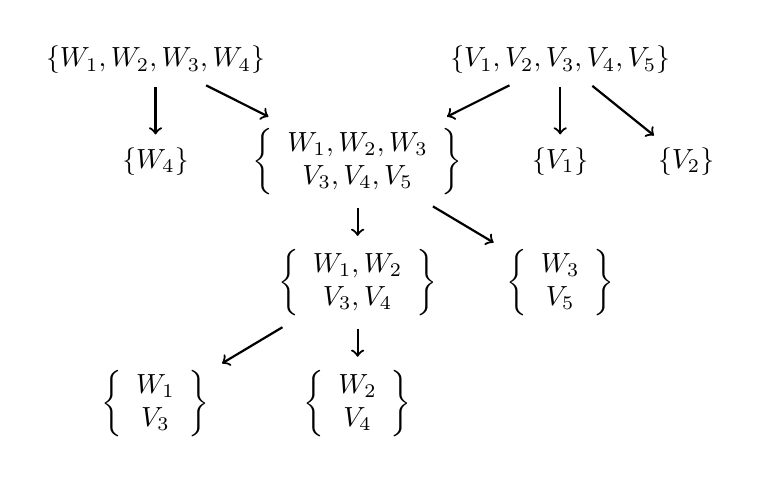
\begin{tikzpicture}[thick,shorten >=1pt, shorten <=1pt,->]
%  \matrix (m) [matrix of math nodes, row sep=3em, column sep={5em,between origins}]{
  \matrix (m) [matrix of math nodes, row sep=1.3em, column sep=-1.1em]{
	 \{W_1,W_2,W_3,W_4\} & & \{V_1,V_2,V_3,V_4,V_5\} & \\
	\{W_4\} & \left\{ \begin{array}{c} W_1,W_2,W_3 \\ V_3,V_4,V_5 \end{array} \right\} & \{V_1\} & \{V_2\} \\
	& \left\{\begin{array}{c} W_1,W_2 \\ V_3,V_4 \end{array}\right\} & \left\{ \begin{array}{c} W_3 \\ V_5 \end{array} \right\}\\
	\left\{ \begin{array}{c} W_1 \\ V_3 \end{array} \right\}  & \left\{ \begin{array}{c} W_2 \\ V_4 \end{array} \right\} & \\
  };
  \path 
  	(m-1-1) edge (m-2-1)
  	(m-1-1) edge (m-2-2)
  	(m-1-3) edge (m-2-2)
  	(m-1-3) edge (m-2-3)
  	(m-1-3) edge (m-2-4)
  	(m-2-2) edge (m-3-2)
  	(m-2-2) edge (m-3-3)
  	(m-3-2) edge (m-4-1)
  	(m-3-2) edge (m-4-2)
  ;
\end{tikzpicture}
\end{document}
}
\vspace*{-2ex}
\caption{\label{fig:multitree} The projection signature graph of Example~\ref{exa:basic}.}
\end{figure}
%
Note that in the figure we have collapsed equivalent attributes in a unique equivalence class, according to the renaming schema. Furthermore, since all its projection constructs have $q=1$, this knowledge base belongs to \DLRpm.
%\todo{maybe add an axiom that breaks this multi-tree feature?}
%
%In addition to the above multitree condition, the \DLRpm fragment of \DLRp allows for knowledge bases with projection constructs $\EXISTR{q}{U_1,\ldots,U_k} R$ (resp. $\EXISTR{q}{U} R$) with a cardinality $q>1$ only if the length of the path $\pth{\{U_1,\ldots,U_k\}}{\tau(R)}$ (resp. $\pth{\{U\}}{\tau(R)}$) is 1.

\DLR is included in \DLRpm, since the projection signature graph of any \DLR knowledge base is always a degenerate multitree with maximum depth equal to 1. 
%
Not all the database constraints as introduced in Section~\ref{sec:expressivity} can be directly expressed in \DLRpm. Equijoins, external uniqueness axioms, and identification axioms introduce projections which share common attributes, thus violating the multitree restriction. However, it is still possible to express in \DLRpm external uniqueness and identification axioms by encoding them as a special set of ABox axioms, as originally proposed in~\cite{CalvaneseGL01}. Therefore, we can conclude that \DLRID~\cite{CalvaneseGL01} extended with unary functional dependencies is included in \DLRpm{}\negmedspace, provided that projections of relations in the knowledge base form a multitree projection signature graph. Since (unary) functional dependencies are expressed via the inclusions of projections of relations, by constraining the projection signature graph to be a multitree, the possibility to build combinations of functional dependencies as the ones in~\cite{CalvaneseGL01} leading to undecidability is ruled out.

Concerning the ability of \DLRpm to capture conceptual data models, only the mapping of ORM schemas is affected by the \DLRpm restrictions: \DLRpm is able to correctly express an ORM schema if the projections involved in the schema satisfy the \DLRpm multitree restriction.

%%%%%%%%%%%%%%%%%%%%%%%%%%%%%%%%%%%%%%%%%%%%%%%%%%%%%%%%%%%%%%%%%%%%%%
%%%%%%%%%%%%%%%%%%%%%%%%%%%%%%%%%%%%%%%%%%%%%%%%%%%%%%%%%%%%%%%%%%%%%%

\begin{figure}
	[t] 
	\centering
%		\renewcommand{\arraystretch}{1.2} 
		\resizebox{\columnwidth}{!}{
		$ 
		\begin{array}{r@{\hspace{1ex}}c@{\hspace{1ex}}l} 
			(\neg C)^\dag &=& \neg C^\dag \\
			%
			(C_1 \sqcap C_2)^\dag & =& C_1^\dag \sqcap C_2^\dag \\
			%
			(C_1 \sqcup C_2)^\dag & =& C_1^\dag \sqcup C_2^\dag \\
			%
			(\EXISTR{q}{U_i} R)^\dag & =& \card{q}{\left(\pth{\tau(R)}{\{U_i\}}^\dag\right)^-}{R^\dag}\\
			%
			(\greif{R})^\dag &=& R^\dag \\
			%
			(\lreif{R\!N})^\dag &=& A^l_{R\!N}
			%
			%
			\vspace{2ex}\\
			%
			%
			(R_1\setminus R_2)^\dag &=& R_1^\dag\sqcap \neg R_2^\dag\\
			%
			(R_1 \sqcap R_2)^\dag & =& R_1^\dag \sqcap R_2^\dag\\
			%
			(R_1 \sqcup R_2)^\dag & =& R_1^\dag \sqcup R_2^\dag\\
			%
			(\selects{U_i}{C}{R})^\dag & =& R^\dag \sqcap \forall \pth{\tau(R)}{\{U_i\}}^\dag \per C^\dag\\
			%
			(\EXISTR{q}{U_1,\ldots,U_k} R)^\dag & =&
			%  \begin{cases}
			%    {R^\dag} & \parbox[t]{\textwidth}{$\text{if } q=1 \text{ and }\\ \{U_1,\ldots,U_k\}\!=\!\tau(R)$}\\
			\card{q}{\left(\pth{\tau(R)}{\{U_1,\ldots,U_k\}}^\dag\right)^-}{R^\dag} 
			%    & \text{otherwise}
			% \end{cases}                                   
		\end{array}
		$ 
		}
%		\renewcommand{\arraystretch}{1} 
		\vspace*{-2ex}
	\caption{The mapping for concept and relation expressions.} \label{fig:themapping}
\end{figure}
%

\section{Mapping \DLRpm to \ALCQI}
\label{sec:mapping}

We show that reasoning in \DLRpm is \ExpTime-complete, using the \ExpTime-completeness of 
\ALCQI~\cite{BCMNP03}, by providing a mapping from \DLRpm KBs to \ALCQI KBs, and by observing that \ALCQI is directly expressible in \DLR.
%
We adapt and extend the mapping presented for \DLR in~\cite{Calvanese:et:al:TOCL-2008}, with the modifications proposed by~\cite{HorrocksSTT00} to deal with ABoxes without the unique name assumption.

%We quickly remind that \ALCQI \emph{concepts} $C$ and \emph{roles} $S$ are defined as follows:
%%
%\begin{align*}
%C  &\to \top\ \mid\ \bot\  \mid\ A_i ~\mid~  \neg C ~\mid~ C_1 \sqcap C_2
%~\mid~ C_1 \sqcup C_2 ~\mid~ \card{q}{S_i}{C} ~\mid~
%\forall S_i\per C,\\
%S &\to Q_i\ \mid Q_i^-,
%\end{align*}
%%
%where $A_i$ is a concept name and $Q_i$ a role name. The non-boolean constructors are interpreted in an interpretation $\mathcal{I} = (\Delta,\Int \cdot)$ by taking
%%
%\begin{align*}
%  (\card{q}{S_i}{C})^\mathcal{I} &= \{ x\in\Delta \mid~\left|\{y\in
%                  \Delta \mid
%                  (x,y)\in S_i^\mathcal{I} \wedge y\in C^\mathcal{I}\}\right| \lesseqgtr q \},\\
%%
%  (\forall S_i\per C)^\mathcal{I} &= \{ x\in\Delta \mid \forall y\in \Delta\
%                                 ((x,y)\in S_i^\mathcal{I} \to y\in C^\mathcal{I}) \},\\
%%
%  \Int{(Q_i^-)} &= \{(x,y)\in \Delta\times \Delta \mid (y,x)\in \Int
%Q\}.
%\end{align*}

In the following $(S_1\chain\ldots\chain S_n)^-$ stands for $S_n^-\chain\ldots\chain S_1^-$, $\exists^{\lesseqgtr 1} S_1\chain\ldots\chain S_n\per C$ stands for $\card{1}{S_1\per\ldots\per\exists^{\lesseqgtr 1} S_n}{C}$, and $\forall S_1\chain\ldots\chain S_n\per C$ for $\forall S_1\per\ldots\per\forall S_n\per {C}$. The concept expressions $\exists^{\lesseqgtr 1}\bot\per{C}$ and $\forall \bot\per {C}$ stand for the $\bot$ concept.
%Note that the
%shortcut for qualified number restrictions holds for the case
%$q=1$.
%
% for the role chain constructor ``$\chain$'' are not correct
% in general, but they are correct in the context of the specific \ALCQI
% knowledge bases used in this paper.
%
For a relation instance axiom %in the ABox 
of the form
$R\!N(U_1\!:\!o_1,\ldots,U_n\!:\!o_n)$ we use the shortcut $R\!N(t)$,
with $t = \langle U_1\!:\!o_1,\ldots,U_n\!:\!o_n\rangle$ a
\emph{relation instance}, i.e., a $\mathcal{U}$-labelled tuple over $\Ob$.

Let $\KB = (\mathcal{T},\A,\Re)$ be a \DLRpm KB.
We first pre-process \KB by transforming it into a logically equivalent one as follows: for each equivalence class 
$[U]_{\Re}$ a single \emph{canonical} representative of the class is chosen, and \KB is consistently rewritten by 
substituting each attribute with its canonical representative. 
After this rewriting, the renaming schema does not play any role in the mapping.

%%%%%%%%%%%%%%%%%%%%%%%%%%%


We first introduce a mapping function $\cdot^\dag$ from \DLRpm
concepts and relations to \ALCQI concepts. 
%Starting with atomic expressions, t
The function $\cdot^\dag$ maps each
concept name $C\!N$ and each relation name $R\!N$ appearing in the \DLRpm KB to an \ALCQI concept
name $C\!N$ and $A_{R\!N}$, respectively. The latter is the global reification of $R\!N$.
%
For each relation name $R\!N$, the \ALCQI signature also
includes a concept name $A_{R\!N}^{l}$ and a role name $Q_{R\!N}$that captures local objectification. 
The mapping $\cdot^\dag$
is extended to concept and relation expressions as in
Figure~\ref{fig:themapping}.
%

The mapping crucially uses the projection signature graph structure to map projections and selections, by accessing paths in the projection signature $\mathscr{T}$ associated to the \DLRpm KB. If there is a path $\pth{\tau}{\tau'} = \tau,\tau_1,\ldots,\tau_n, \tau'$ from ${\tau}$ to ${\tau'}$ in $\mathscr{T}$, then its mapping is the \ALCQI role chain expression using role names $Q_{\tau_i}$:
%
\[
	\pth{\tau}{\tau'}^\dag = Q_{\tau_1}\chain\ldots\chain Q_{\tau_n}\chain Q_{\tau'}. 
\]
%
with $\pth{\tau}{\tau'}^\dag = \bot$ if $\pth{\tau}{\tau'} = \emptyset$.
%
%Furthermore, the \ALCQI signature also includes a role name $Q_{\tau_i}$ for each projected signature $\tau_i$ in the projection signature, $\tau_i\in\mathscr{T}$, such that there exists $\tau_j\in\mathscr{T}$ with $\chd{\tau_j}{\tau_i}$, i.e., we exclude the case where $\tau_i$ is one of the roots of the multitree induced by the projection signature.
%

We also include a concept name $A_{R\!N}^{\tau_i}$ for each projected signature $\tau_i$ in the projection signature graph dominated by $\tau(R\!N)$, $\tau_i\in\mathscr{T}_{\tau(R\!N)}$ to capture global reifications of the projections of $R\!N$. Note that $A_{R\!N}^{\tau(R\!N)}$ coincides with $A_{R\!N}$.

Intuitively, the mapping reifies each node in the projection signature graph: the target \ALCQI signature of 
Example~\ref{exa:basic} is partially presented in Fig.~\ref{fig:mapping}, together with the projection signature graph. 
Each node is labelled with the corresponding global reification concept ($A_{R_i}^{\tau_j}$), for each %relation name 
$R_i\in\mathcal{R}$ and each projected signature $\tau_j$ in the projection signature graph dominated by $\tau(R_i)$, 
while the edges are labelled by the roles ($Q_{\tau_i}$) needed for the reification.
%
\begin{figure}[t]
\centering
%\tikz[x=6em,y=10ex] {\tiny
%\node (a) at (2,3)  {$A_{R_1}, A_{R_2}$};
%\node (b) at (4,3)  {$A_{R_3}$};
%\node (c) at (1,2)  {$A_{R_1}^{\{U_1,U_2\}}, A_{R_2}^{\{U_1,U_2\}}$};
%\node (c1) at (5,1)  {$A_{R_1}^{\{U_5\}}, A_{R_2}^{\{U_5\}}, A_{R_3}^{\{U_5\}}$};
%\node (d) at (3,2)  {$A_{R_1}^{\{U_3,U_4,U_5\}}, A_{R_2}^{\{U_3,U_4,U_5\}}, A_{R_3}^{\{U_3,U_4,U_5\}}$};
%\node (d1) at (5,2)  {$A_{R_3}^{\{W_4\}}$};
%\node (e) at (0,1)  {$A_{R_1}^{\{U_1\}}, A_{R_2}^{\{U_1\}}$};
%\node (f) at (1,1)  {$A_{R_1}^{\{U_2\}}, A_{R_2}^{\{U_2\}}$};
%\node (g) at (3,1)  {$A_{R_1}^{\{U_3,U_4\}}, A_{R_2}^{\{U_3,U_4\}}, A_{R_3}^{\{U_3,U_4\}}$};
%\node (h) at (2,0)  {$A_{R_1}^{\{U_3\}}, A_{R_2}^{\{U_3\}}, A_{R_3}^{\{U_3\}}$};
%\node (i) at (4,0)  {$A_{R_1}^{\{U_4\}}, A_{R_2}^{\{U_4\}}, A_{R_3}^{\{U_4\}}$};
%\node (ac) at (1.3,2.7) {$Q_{{\{U_1,U_2\}}}$};
%\node (ad) at (2.75,2.7) {$Q_{\{U_3,U_4,U_5\}}$};
%\node (bd) at (4,2.5) {$Q_{\{U_3,U_4,U_5\}}$};
%\node (bd1) at (4.75,2.5) {$Q_{\{W_4\}}$};
%\node (ce) at (0.3,1.6) {$Q_{{\{U_1\}}}$};
%\node (cf) at (1.23,1.6) {$Q_{{\{U_2\}}}$};
%\node (dg) at (2.7,1.6) {$Q_{{\{U_3,U_4\}}}$};
%\node (dc1) at (4.2,1.6) {$Q_{{\{U_5\}}}$};
%\node (gh) at (2.2,0.5) {$Q_{\{U_3\}}$};
%\node (gi) at (3.75,0.5) {$Q_{\{U_4\}}$};
%\draw 
%(a) edge[->] (c)
%(a) edge[->] (d)
%(d) edge[->] (c1)
%(b) edge[->] (d)
%(b) edge[->] (d1) 
%(c) edge[->] (e)
%(c) edge[->] (f) 
%(d) edge[->] (g)
%(g) edge[->] (h) 
%(g) edge[->] (i);
%}
%\end{center}
%\vspace*{-2mm}
\resizebox{\columnwidth}{!}{
\documentclass[tikz]{standalone}

\usetikzlibrary{matrix,positioning}
\begin{document}

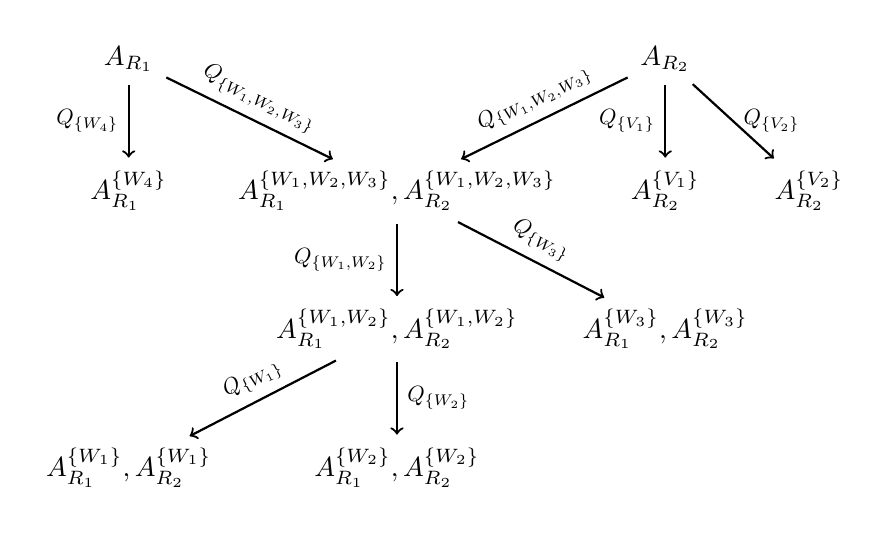
\begin{tikzpicture}[thick,shorten >=1pt, shorten <=1pt,->]
%  \matrix (m) [matrix of math nodes, row sep=3em, column sep={5em,between origins}]{
  \matrix (m) [matrix of math nodes, row sep=2.9em, column sep=0.3em]{
	 A_{R_1} & & A_{R_2} & \\
	A_{R_1}^{\{W_4\}} & A_{R_1}^{\{W_1,W_2,W_3\}},A_{R_2}^{\{W_1,W_2,W_3\}} & A_{R_2}^{\{V_1\}} & A_{R_2}^{\{V_2\}} \\
	& A_{R_1}^{\{W_1,W_2\}},A_{R_2}^{\{W_1,W_2\}} & A_{R_1}^{\{W_3\}},A_{R_2}^{\{W_3\}}\\
	A_{R_1}^{\{W_1\}},A_{R_2}^{\{W_1\}}  & A_{R_1}^{\{W_2\}},A_{R_2}^{\{W_2\}} \\
  };
  \path 
  	(m-1-1) edge node[left] {\scalebox{0.8}{$Q_{\{W_4\}}$}} (m-2-1)
  	(m-1-1) edge node[above right,sloped,anchor=south] {\scalebox{0.8}{$Q_{\{W_1,W_2,W_3\}}$}} (m-2-2)
  	(m-1-3) edge node[above right,sloped,anchor=south] {\scalebox{0.8}{$Q_{\{W_1,W_2,W_3\}}$}} (m-2-2)
  	(m-1-3) edge node[left] {\scalebox{0.8}{$Q_{\{V_1\}}$}} (m-2-3)
  	(m-1-3) edge node[right] {\scalebox{0.8}{$Q_{\{V_2\}}$}} (m-2-4)
  	(m-2-2) edge node[left] {\scalebox{0.8}{$Q_{\{W_1,W_2\}}$}} (m-3-2)
  	(m-2-2) edge node[right,sloped,anchor=south] {\scalebox{0.8}{$Q_{\{W_3\}}$}} (m-3-3)
  	(m-3-2) edge node[left,sloped,anchor=south] {\scalebox{0.8}{$Q_{\{W_1\}}$}} (m-4-1)
  	(m-3-2) edge node[right] {\scalebox{0.8}{$Q_{\{W_2\}}$}} (m-4-2)
  ;
\end{tikzpicture}
\end{document}
}
\vspace*{-4.5ex}
\caption{\label{fig:mapping} The \ALCQI signature generated by \Texa.}
\end{figure} 

%%%%%%%%%%%%%%%%%%%%%%%%%%%

Recall that \DLRpm restricts to $q=1$ the cardinalities on any path of length greater than $1$.
Thus, we
remain within \ALCQI when the mapping applies to
cardinalities. If we need to express e.g.\ the cardinality constraint
$\EXISTR{q}{U_i} R$ %(or $\EXISTR{q}{U_1,\ldots,U_k} R$), 
with $q>1$,
then $U_i$ %($\{U_1,\ldots,U_k\}$) 
should not be mentioned in any other
projection of the relation $R$ in such a way that
$|\pth{\tau(R)}{\{U_i\}}|=1$. %($|\pth{\tau(R)}{\{U_1,\ldots,U_k\}}|=1$).

In order to explain the need for the path function in the mapping,
notice that a relation is reified according to the decomposition
dictated by the projection signature graph it dominates. Thus, to
access an attribute $U_j$ of a relation ${R_i}$ it is necessary to
follow the path through the projections that use that attribute. This
path is a role chain from the signature of the relation (the root) to
the attribute as returned by the $\pth{\tau(R_i)}{U_i}$ function. For
example, in Figure~\ref{fig:mapping} in order to access the
attribute $U_4$ of the relation $R_3$ in the expression
$(\selects{U_4}{C}{R_3})$, the path $\pth{\tau(R_3)}{\{U_4\}}^\dag$ is
equal to the role chain
$Q_{\{U_3,U_4,U_5\}}\chain Q_{\{U_3,U_4\}}\chain Q_{\{U_4\}}$, so that
$ (\selects{U_4}{C}{R_3})^\dag ~=~ A_{R_3} \sqcap \forall
Q_{\{U_3,U_4,U_5\}}\chain Q_{\{U_3,U_4\}}\chain Q_{\{U_4\}}\per C.  $
%\\
Similar considerations can be done when mapping cardinalities over
relation projections.

Let $\KB = (\Tmc, \A)$ be a \DLRpm KB with signature
$(\mathcal{C},\mathcal{R},\mathcal{U},\tau)$. The mapping
$\gamma(\KB) = (\gamma(\Tmc),\gamma(\A))$ defines the
\ALCQI KB:
%
\begin{align*}
  \gamma(\Tmc)  = {} &  \gamma_{\textit{dsj}} ~\cup %
  \bigcup_{R\!N\in\Rmc}\gamma_{\textit{rel}}(R\!N) ~\cup %
  \bigcup_{R\!N\in\Rmc}\gamma_{\textit{lobj}}({R\!N})
  ~\cup \\
%  \bigcup_{{R\!N}\in\Rmc, P_i\in \mathscr{T}_{R\!N}}\hspace*{-1.7em}\gamma_{\textit{part}}({P_i})\quad\cup\quad %
% \bigcup_{U_1\looparrowright U_2\in\KB}\hspace*{-1em}{U_1 \equiv U_2}\quad\cup\quad %
  & \bigcup_{C_1\sqsubseteq C_2\in\KB}{C_1^\dag\sqsubseteq C_2^\dag}
  ~\cup%
 \bigcup_{R_1\sqsubseteq R_2\in\KB}{R_1^\dag\sqsubseteq
    R_2^\dag},%
\end{align*}
%
where
\vspace{-1ex}
%
\begin{align*}
\gamma_\textit{dsj} = {} % &~\bigl\{A\sqsubseteq\neg A_{R\!N}
  % \mid A\in\Cmc ~\mbox{and}~ {R\!N}\in\Rmc\bigr\} ~\cup \\
&~\bigl\{A_{R\!N_1}^{\tau_i}\sqsubseteq\neg A_{R\!N_2}^{\tau_j} \mid R\!N_1, R\!N_2\in\Rmc, \\
 & \qquad \qquad \tau_i, \tau_j\in \mathscr{T}, |\tau_i|\geq 2, |\tau_j|\geq 2, \tau_i\neq \tau_j
  \bigr\}\\
% &\bigl\{{R\!N_1^\dag}\sqsubseteq\neg {R\!N_2^\dag} \mid R\!N_1, R\!N_2\in\Rmc,
%   \exists P_i\in \mathscr{T}_{R\!N_1}\per \forall P_j\in \mathscr{T}_{R\!N_2}\per [P_i]_{\Re} \neq [P_j]_{\Re}
%   \bigr\};\\
%note that $A_2^\dag$ includes also all the concepts names of the form $A_{R\!N}^{P_i}$;
%
  \gamma_{\textit{rel}}(R\!N) =&~\bigcup_{\mathclap{\tau_i\in\mathscr{T}_{\tau(R\!N)}}}\quad
     \bigcup_{\mathrlap{\chd{\tau_i}{\tau_j}}}\bigl\{
     A^{\tau_i}_{R\!N} \sqsubseteq \exists Q_{\tau_j}\per A^{\tau_j}_{R\!N},~\exists^{\geq 2}
     Q_{\tau_j}\per\top\sqsubseteq \bot
     \bigr\} \\
% ~\cup\\
% &\bigcup_{\textit{child}(\tau_i,U_j)}\hspace*{-1.5em}\bigl\{
%    A^{P_i}_{R\!N} \sqsubseteq \exists {U_j}\per\top,~\exists^{\geq 2}
%    {U_j}\per\top\sqsubseteq \bot\bigr\}\Bigr);\\
%
\gamma_{\textit{lobj}}({R\!N}) =&~\{\parbox[t]{\textwidth}{$
A_{R\!N}\sqsubseteq\exists Q_{R\!N}\per A_{R\!N}^l,~
\exists^{\geq 2}Q_{R\!N}\per \top\sqsubseteq \bot,\\
A_{R\!N}^l \sqsubseteq \exists Q_{R\!N}^-\per A_{R\!N},~
\exists^{\geq 2} Q_{R\!N}^-\per \top\sqsubseteq \bot\}.$}
\end{align*}
%
Intuitively, $\gamma_\textit{dsj}$ ensures that relations with different signatures are disjoint, thus, e.g., enforcing the union compatibility. The axioms in $\gamma_{\textit{rel}}$ introduce classical reification axioms for each relation and its relevant projections. The axioms in $\gamma_{\textit{lobj}}$ make sure that each local objectification differs form the global one.

To translate the ABox, we first map each individual $o$ in the \DLRpm ABox to an \ALCQI individual $o$. % using the identity function.
%
Each relation instance occurring in \A 
%(we say that a relation
%instance $t$ \emph{occurs} in \A if $R\!N(t)\in\A$ for some relation
%name $R\!N$) 
is mapped via an injective function $\xi$ to a distinct
individual. That is, $\xi: T_\Ob(\mathcal{U})\to \mathcal{O}_\ALCQI$,
with $\mathcal{O}_\ALCQI = \Ob\cup \Ob^t$ being the set of individuals
in $\gamma(\KB)$, $\Ob \cap \Ob^t = \emptyset$ and
\vspace{-1.5ex}
$$\xi(t)  ~=~ %\left\{
                  \begin{cases}
                    o\in\Ob, &\text{if } t = \langle U\!:\!o\rangle \\
                    o\in\Ob^t, &\text{otherwise.}\\
                  \end{cases}
$$
%
Following~\cite{HorrocksSTT00}, the mapping $\gamma(\A)$ in Figure~\ref{fig:gammaA} introduces a new concept name $Q_o$ for each individual in $o \in\Ob$ and a new concept name $Q_t$ for each relation instance occurring in \A,
%
\begin{figure}[t]
\resizebox{\columnwidth}{!}{\parbox{1.198\columnwidth}{
\begin{align}
\gamma(\A) =
& \label{eq:ob1}
\{ C\!N^\dag(o) \mid C\!N(o)\in\A \} ~\cup\\
& \label{eq:ob2}
\{ o_1\neq o_2 \mid o_1\neq o_2\in\A \} ~\cup~\{ o_1=o_2 \mid o_1= o_2\in\A \}~\cup\\
& \label{eq:rei1}
\{A^{\tau_i}_{R\!N}(\xi(t[\tau_i])) \mid R\!N(t)\in\A \textit{ and } \tau_i
  \in\mathscr{T}_{\tau(R\!N)}\} ~\cup\\
& \label{eq:rei2}
\{ Q_{\tau_j}\big(\xi(t[\tau_i]),\xi(t[\tau_j])\big) \mid
  \chd{\tau_i}{\tau_j} \}\\
& \label{eq:unique1}
\{Q_o(o)\mid o\in\Ob\}~\cup\\
& \label{eq:unique2}
\{Q_t(o_1), Q_t\sqsubseteq C_t \mid t = \langle
  U_1\!:\!o_1,\ldots, U_n\!:\!o_n\rangle \text{ occurs in } \A\},
\end{align}
}}
\vspace*{-2.5ex}
\caption{The mapping $\gamma(\A)$}
\label{fig:gammaA}
\end{figure}
%
where $C_t$ stands for the concept

\noindent
\resizebox{\columnwidth}{!}{
\parbox{1.17\columnwidth}{
\begin{align*}
%  \label{eq:unique3}
  & \exists^{\leq 1}\big(\pth{\tau(t)}{\{U_1\}}^\dag
  \big)^-.  \\[-1mm] & ~~\exists \big(\pth{\tau(t)}{\{U_2\}}^\dag
  \big). Q_{o_2}\sqcap\ldots\sqcap 
  \exists \big(\pth{\tau(t)}{\{U_n\}}^\dag
  \big). Q_{o_n}~~.
\end{align*}
}}
%
Intuitively, \eqref{eq:rei1} and \eqref{eq:rei2} reify each relation
instance occurring in \A using the projection signature of the
relation instance itself. The formulas \eqref{eq:unique1}-\eqref{eq:unique2} guarantee that there is exactly one \ALCQI
individual reifying a given relation instance.
%
Clearly, the size of $\gamma(\KB)$ is polynomial in the size of $\KB$
under the same coding of the numerical parameters. \\
%
We are able to state our main results.

\begin{theorem}
	\label{th:sat} A \DLRpm knowledge base $\KB$ is satisfiable iff the \ALCQI knowledge base $\gamma(\KB)$ is satisfiable. 
\end{theorem}
%
As a direct consequence of this theorem and the fact that \DLR is a sublanguage of \DLRpm, we obtain the following.

\begin{corollary}
  Reasoning in \DLRpm is \ExpTime-complete.
\end{corollary}


%%%%%%%%%%%%%%%%%%%%%%%%%%%%%%%%%%%%%%%%%%%%%%%%%%%%%%%%%%%%%%%%%%%%%%
%%%%%%%%%%%%%%%%%%%%%%%%%%%%%%%%%%%%%%%%%%%%%%%%%%%%%%%%%%%%%%%%%%%%%%
\section{Implementation of a \DLRpm API}

We have implemented the framework discussed in this paper. DLRtoOWL is a Java-based library which fully implements \DLRpm language services. The library is based on the tool ANTLR4 to parse serialised input provided by the user, and on OWLAPI4 for the OWL2 encoding. The final user could define its own knowledge base in a text file, or via a \textsc{tell} interface, on which an algorithm constructing the multitree is applied. After that, the tool performs the encoding into OWL. The system includes JFact, the Java-based version of the popular Fact++ reasoner. DLRtoOWL provides the most used reasoning services (hierarchy, satisfiability, entailment, etc.) via a \textsc{ask} interface. In DLRtoOWL we also provide a Java DLRApi package to allow developers to create, manipulate and serialise \DLRpm knowledge bases in their Java-based application, extending in a compatible way the standard OWL API.

During development we strongly focused on performance. Since the OWL encoding is only possible if we have already built the multitree, ideally the program should performs two parsing rounds: one for the creating of the multitree and the other one for the OWL mapping. We faced this issue using dynamic programming: during the first (and only) parsing round we store in a data structure each axiom that we want to translate in OWL, and after building the tree, by the dynamic programming technique we build on-the-fly a Java class which generates the required axioms.

%%%%%%%%%%%%%%%%%%%%%%%%%%%%%%%%%%%%%%%%%%%%%%%%%%%%%%%%%%%%%%%%%%%%%%
\section{Conclusions}

We have introduced the very expressive description logic \DLRp{}\negmedspace, which extends \DLR with constructors capable of dealing with database oriented constraints. In particular, this logic is expressive enough to cover directly and more thoroughly the EER, UML, and ORM conceptual data models, among others.

Although reasoning in \DLRp is undecidable, we show that a simple syntactic constraint on KBs restores decidability. In fact, the resulting logic \DLRpm has the same complexity (\ExpTime-complete) as the basic \DLR language. In other words, handling database constraints does not increase the complexity of reasoning in these logics.

To enhance the use and adoption of \DLRpm, we have developed an API that fully implements
this language, and maps input KBs into OWL. Using a standard OWL reasoner, we are able to
provide a variety of \DLRpm reasoning services as well. 

\todo[inline]{Something about future work?}

%%%%%%%%%%%%%%%%%%%%%%%%%%%%%%%%%%%%%%%%%%%%%%%%%%%%%%%%%%%%%%%%%%%%%%

%%%%% Blind!
%\section{Acknowledgements}
%We thank Alessandro Mosca for working with us on all the preliminary work necessary to understand how to get these technical results.

%%%%%%%%%%%%%%%%%%%%%%%%%%%%%%%%%%%%%%%%%%%%%%%%%%%%%%%%%%%%%%%%%%%%%%
%%%%%%%%%%%%%%%%%%%%%%%%%%%%%%%%%%%%%%%%%%%%%%%%%%%%%%%%%%%%%%%%%%%%%%

\cleardoublepage
\bibliographystyle{named}
%%\bibliography{short-string,krdb}
\bibliography{biblio}

%%%%%%%%%%%%%%%%%%%%%%%%%%%%%%%%%%%%%%%%%%%%%%%%%%%%%%%%%%%%%%%%%%%%%%
%%%%%%%%%%%%%%%%%%%%%%%%%%%%%%%%%%%%%%%%%%%%%%%%%%%%%%%%%%%%%%%%%%%%%%
%%%%%%%%%%%%%%%%%%%%%%%%%%%%%%%%%%%%%%%%%%%%%%%%%%%%%%%%%%%%%%%%%%%%%%

\end{document}

%%% Local Variables:
%%% mode: latex
%%% TeX-master: t
%%% save-place: t
%%% End:
